\documentclass[tikz,border=14pt]{standalone}
\usepackage{amsmath,amssymb}
\usepackage{microtype}
\usepackage[scaled=0.92]{helvet}
\renewcommand{\familydefault}{\sfdefault}
\usepackage{tikz}
\usetikzlibrary{
  arrows.meta,
  backgrounds,
  calc,
  positioning,
  shapes.geometric
}

% ==============================================================================
% PTIT SIGNATURE COLOR PALETTE
% ==============================================================================
\definecolor{PTITred}{HTML}{C96A78}       % Dusty pastel red (PTIT signature)
\definecolor{BlushPink}{HTML}{E8B8BE}     % Accent nhe
\definecolor{MutedMauve}{HTML}{B89AA5}    % Secondary
\definecolor{WarmIvory}{HTML}{FAF8F6}     % Neutral chinh
\definecolor{SoftCharcoal}{HTML}{3F4146}  % Text
\definecolor{CoolGray}{HTML}{C9CDD2}      % Line / border
\definecolor{DustyBlue}{HTML}{AABCC8}     % Highlight phu

% Soft harmonious tints
\colorlet{RedTint}{PTITred!15}
\colorlet{RedSoft}{PTITred!28}
\colorlet{BlueTint}{DustyBlue!25}
\colorlet{BlueSoft}{DustyBlue!45}
\colorlet{MauveTint}{MutedMauve!22}
\colorlet{PinkTint}{BlushPink!30}
\colorlet{BorderColor}{CoolGray!85}

\begin{document}
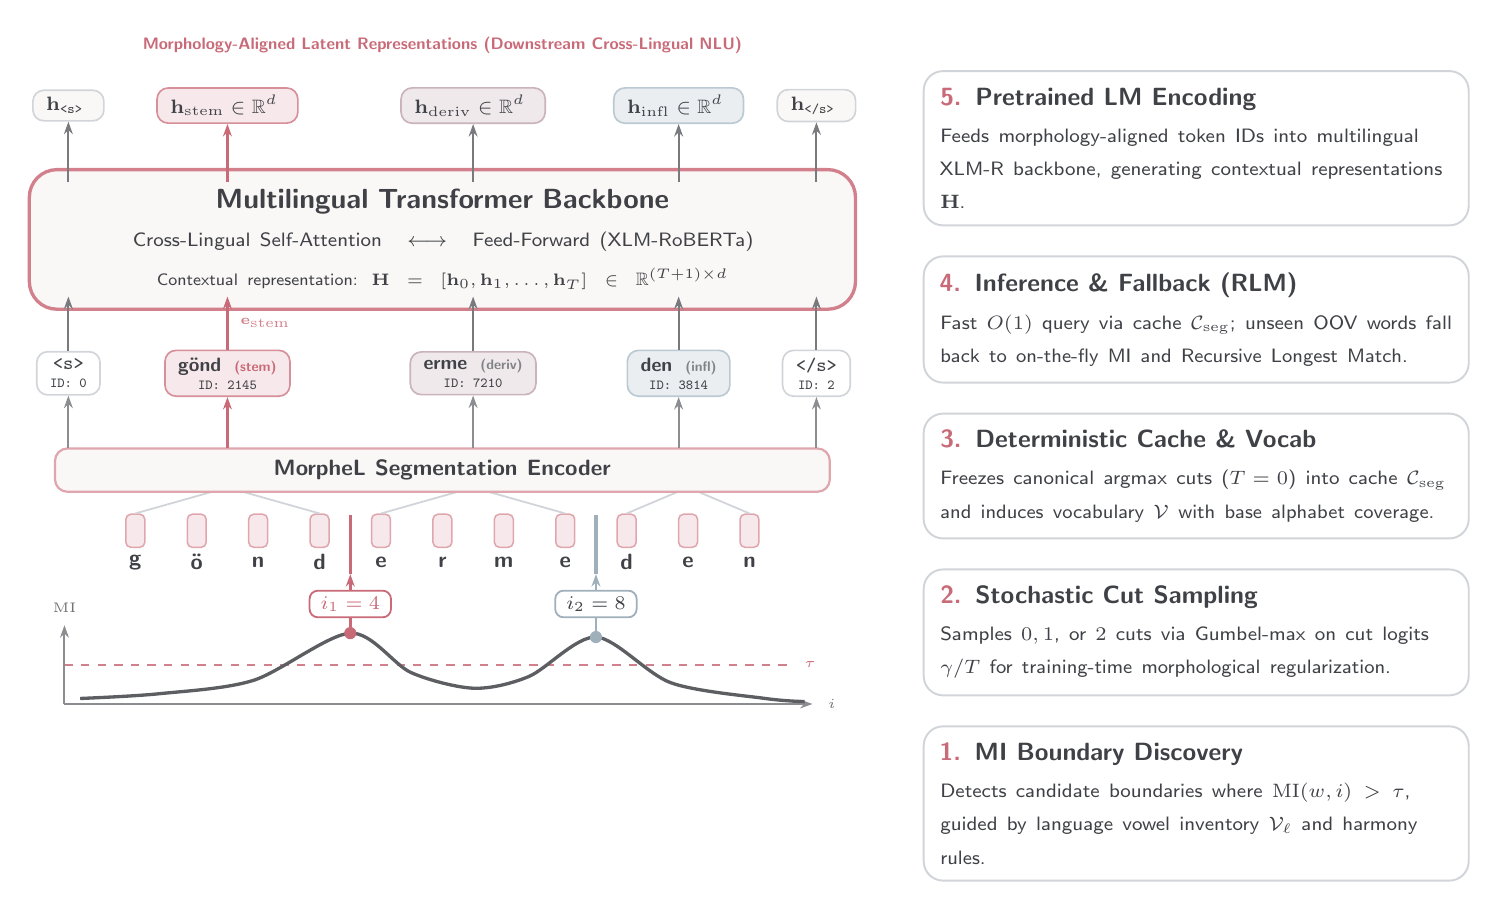
\begin{tikzpicture}[
  font=\sffamily,
  text=SoftCharcoal,
  >={Stealth[length=4.5pt, width=3.2pt]},
  line width=0.8pt,
  % --- Reusable Minimalist Styles (BLT & MEGABYTE paradigm) ---
  callout/.style={
    draw=BorderColor,
    line width=0.7pt,
    fill=white,
    rounded corners=7pt,
    inner sep=6.0pt,
    text width=6.5cm
  },
  pill/.style={
    draw=BorderColor,
    line width=0.6pt,
    rounded corners=4pt,
    inner xsep=4.8pt,
    inner ysep=2.6pt,
    font=\sffamily\scriptsize,
    align=center
  },
  bytebar/.style={
    draw=PTITred!60,
    line width=0.55pt,
    fill=RedTint,
    rounded corners=1.8pt,
    minimum width=2.4mm,
    minimum height=4.2mm,
    inner sep=0pt
  },
  mainbackbone/.style={
    draw=PTITred!85,
    line width=1.2pt,
    fill=WarmIvory,
    rounded corners=10pt,
    inner sep=7pt
  }
]

% ==============================================================================
% HORIZONTAL RECTANGULAR ARCHITECTURE (ASPECT RATIO ~ 2.15 : 1)
% Pure Neural Architecture (BLT & MEGABYTE Paradigm, Zero Box Engineering)
% Spacious, Airy Vertical Rhythm (Generous Breathing Room)
% Dimensions: ~18.8cm width x 9.0cm height (Ideal 2-column paper span)
% ==============================================================================

% ==============================================================================
% LEFT PANEL: NEURAL MORPHEME TOKENIZER PIPELINE (X = 0.5 to 10.5)
% ==============================================================================

% ------------------------------------------------------------------------------
% 1. BOTTOM: MI CURVE & STATISTICAL BOUNDARIES (SPACIOUS & PROMINENT)
% ------------------------------------------------------------------------------
\coordinate (mi_orig) at (0.6, 0.45);

% Threshold dashed line tau
\draw[dashed, draw=PTITred!85, line width=0.8pt] (0.6, 0.95) -- (9.8, 0.95)
  node[right=2pt, font=\tiny\bfseries, text=PTITred] {$\tau$};

% Axes
\draw[->, draw=SoftCharcoal!60, line width=0.7pt] (0.6, 0.45) -- (10.1, 0.45)
  node[right=2pt, font=\tiny, text=SoftCharcoal!75] {$i$};
\draw[->, draw=SoftCharcoal!60, line width=0.7pt] (0.6, 0.45) -- (0.6, 1.45)
  node[above=1pt, font=\tiny, text=SoftCharcoal!75] {$\mathrm{MI}$};

% Characters and byte pills (x-spacing delta = 0.78, centered at 5.4)
% k=0(g):1.50, k=1(o):2.28, k=2(n):3.06, k=3(d):3.84 | cut1=4.23 |
% k=4(e):4.62, k=5(r):5.40, k=6(m):6.18, k=7(e):6.96 | cut2=7.35 |
% k=8(d):7.74, k=9(e):8.52, k=10(n):9.30
\foreach \ch [count=\k from 0] in {g,{\"o},n,d,e,r,m,e,d,e,n} {
  \pgfmathsetmacro{\xpos}{5.4 + (\k - 5) * 0.78}
  \node[font=\footnotesize\bfseries, text=SoftCharcoal] (ch\k) at (\xpos, 2.25) {\ch};
  \node[bytebar] (b\k) at (\xpos, 2.65) {};
}

% Smooth Spline perfectly peaking at cut1 (4.23) and cut2 (7.35)
\draw[line width=1.2pt, draw=SoftCharcoal!85, smooth] plot coordinates {
  (0.8, 0.52)
  (1.8, 0.58)
  (3.0, 0.75)
  (4.23, 1.35)   % Peak 1 (Boundary i1 = 4, exactly between 'd' and 'e')
  (5.0, 0.85)
  (5.8, 0.65)
  (6.5, 0.80)
  (7.35, 1.30)   % Peak 2 (Boundary i2 = 8, exactly between 'e' and 'd')
  (8.3, 0.72)
  (9.5, 0.52)
  (10.0, 0.48)
};

% Peaks circles
\fill[PTITred] (4.23, 1.35) circle (2.2pt);
\fill[DustyBlue!90!SoftCharcoal] (7.35, 1.30) circle (2.2pt);

% Vertical indicator lines from peaks pointing into character boundaries
\draw[->, draw=PTITred, line width=0.9pt] (4.23, 1.35) -- (4.23, 2.10);
\draw[->, draw=DustyBlue!90!SoftCharcoal, line width=0.9pt] (7.35, 1.30) -- (7.35, 2.10);

% Prominent, spacious callout tags for i1 = 4 and i2 = 8 (Floating cleanly in the gap)
\node[fill=white, draw=PTITred, line width=0.65pt, rounded corners=3pt, inner xsep=4pt, inner ysep=2pt, font=\scriptsize\bfseries, text=PTITred]
  at (4.23, 1.72) {$i_1 = 4$};

\node[fill=white, draw=DustyBlue!90!SoftCharcoal, line width=0.65pt, rounded corners=3pt, inner xsep=4pt, inner ysep=2pt, font=\scriptsize\bfseries, text=SoftCharcoal]
  at (7.35, 1.72) {$i_2 = 8$};

% Boundary cut markers between characters
\draw[draw=PTITred, line width=1.2pt] (4.23, 2.10) -- (4.23, 2.85);
\draw[draw=DustyBlue!90!SoftCharcoal, line width=1.2pt] (7.35, 2.10) -- (7.35, 2.85);

% ------------------------------------------------------------------------------
% 2. TOKENIZER ENCODER BAR (SLIM, ELEGANT, SPACIOUS)
% ------------------------------------------------------------------------------

% Funnel grouping lines entering tokenizer bar (length ~5.5mm, clean & distinct)
\draw[draw=BorderColor, line width=0.65pt] (b0.north) -- (2.67, 3.20);
\draw[draw=BorderColor, line width=0.65pt] (b3.north) -- (2.67, 3.20);

\draw[draw=BorderColor, line width=0.65pt] (b4.north) -- (5.79, 3.20);
\draw[draw=BorderColor, line width=0.65pt] (b7.north) -- (5.79, 3.20);

\draw[draw=BorderColor, line width=0.65pt] (b8.north) -- (8.52, 3.20);
\draw[draw=BorderColor, line width=0.65pt] (b10.north) -- (8.52, 3.20);

% Clean horizontal tokenizer bar directly processing byte stream
\node[draw=PTITred!60, fill=WarmIvory, rounded corners=4.5pt, text width=9.7cm, minimum height=5.5mm, align=center, inner sep=2pt] (tok_bar) at (5.4, 3.42) {
  \textbf{\footnotesize MorpheL Segmentation Encoder}
};

% ------------------------------------------------------------------------------
% 3. INDUCED MORPHEME TOKENS (AIRY, GENEROUS ARROW LENGTHS)
% ------------------------------------------------------------------------------

% Morpheme pills emerging from Tokenizer with generous vertical spacing
\node[pill, fill=RedTint, draw=PTITred!75, font=\scriptsize\bfseries] (tok_stem) at (2.67, 4.65) {
  \textsf{g{\"o}nd} \;\textcolor{PTITred}{\tiny(stem)}\\[-1.5pt]
  {\fontsize{5}{6}\selectfont\texttt{ID: 2145}}
};

\node[pill, fill=MauveTint, draw=MutedMauve!75, font=\scriptsize\bfseries] (tok_deriv) at (5.79, 4.65) {
  \textsf{erme} \;\textcolor{SoftCharcoal!65}{\tiny(deriv)}\\[-1.5pt]
  {\fontsize{5}{6}\selectfont\texttt{ID: 7210}}
};

\node[pill, fill=BlueTint, draw=DustyBlue!80, font=\scriptsize\bfseries] (tok_infl) at (8.40, 4.65) {
  \textsf{den} \;\textcolor{SoftCharcoal!65}{\tiny(infl)}\\[-1.5pt]
  {\fontsize{5}{6}\selectfont\texttt{ID: 3814}}
};

% Special tokens
\node[pill, fill=white, draw=BorderColor, font=\scriptsize\bfseries] (tok_s) at (0.65, 4.65) {
  \texttt{<s>}\\[-1.5pt]{\fontsize{5}{6}\selectfont\texttt{ID: 0}}
};
\node[pill, fill=white, draw=BorderColor, font=\scriptsize\bfseries] (tok_e) at (10.15, 4.65) {
  \texttt{</s>}\\[-1.5pt]{\fontsize{5}{6}\selectfont\texttt{ID: 2}}
};

% Generous arrows (length ~9.5mm) from Tokenizer bar into Morpheme Tokens
\draw[->, draw=SoftCharcoal!60, line width=0.7pt] (0.65, 3.70) -- (tok_s.south);
\draw[->, draw=PTITred, line width=0.85pt] (2.67, 3.70) -- (tok_stem.south);
\draw[->, draw=SoftCharcoal!60, line width=0.7pt] (5.79, 3.70) -- (tok_deriv.south);
\draw[->, draw=SoftCharcoal!60, line width=0.7pt] (8.40, 3.70) -- (tok_infl.south);
\draw[->, draw=SoftCharcoal!60, line width=0.7pt] (10.15, 3.70) -- (tok_e.south);

% ------------------------------------------------------------------------------
% 4. CENTRAL PRETRAINED MULTILINGUAL TRANSFORMER BACKBONE
% ------------------------------------------------------------------------------

\node[mainbackbone, text width=10.0cm, minimum height=1.45cm, align=center] (tf_box) at (5.4, 6.35) {
  \textbf{\normalsize Multilingual Transformer Backbone}\\[2pt]
  {\scriptsize Cross-Lingual Self-Attention $\;\longleftrightarrow\;$ Feed-Forward (XLM-RoBERTa)}\\[2pt]
  {\fontsize{6.5}{7.5}\selectfont\textsf{Contextual representation: $\mathbf{H} = [\mathbf{h}_0, \mathbf{h}_1, \dots, \mathbf{h}_T] \in \mathbb{R}^{(T+1) \times d}$}}
};

% Generous arrows (length ~10.5mm) entering Transformer directly from token representations
\draw[->, draw=SoftCharcoal!70, line width=0.75pt] (tok_s.north) -- (0.65, 5.625);
\draw[->, draw=PTITred, line width=0.85pt] (tok_stem.north) -- (2.67, 5.625)
  node[midway, right=1pt, font=\fontsize{5}{6}\selectfont\bfseries, text=PTITred!85] {$\mathbf{e}_{\mathrm{stem}}$};
\draw[->, draw=SoftCharcoal!70, line width=0.75pt] (tok_deriv.north) -- (5.79, 5.625);
\draw[->, draw=SoftCharcoal!70, line width=0.75pt] (tok_infl.north) -- (8.40, 5.625);
\draw[->, draw=SoftCharcoal!70, line width=0.75pt] (tok_e.north) -- (10.15, 5.625);

% ------------------------------------------------------------------------------
% 5. TOP: CONTEXTUAL OUTPUT REPRESENTATIONS (GENEROUS SPACING)
% ------------------------------------------------------------------------------

% Contextual Output Pills with generous vertical distance from Transformer
\node[pill, fill=RedTint, draw=PTITred!75, font=\scriptsize\bfseries] (rep_stem) at (2.67, 8.05) {
  $\mathbf{h}_{\mathrm{stem}} \in \mathbb{R}^d$
};

\node[pill, fill=MauveTint, draw=MutedMauve!75, font=\scriptsize\bfseries] (rep_deriv) at (5.79, 8.05) {
  $\mathbf{h}_{\mathrm{deriv}} \in \mathbb{R}^d$
};

\node[pill, fill=BlueTint, draw=DustyBlue!80, font=\scriptsize\bfseries] (rep_infl) at (8.40, 8.05) {
  $\mathbf{h}_{\mathrm{infl}} \in \mathbb{R}^d$
};

\node[pill, fill=WarmIvory, draw=BorderColor, font=\scriptsize\bfseries] (rep_s) at (0.65, 8.05) {
  $\mathbf{h}_{\text{\tiny\texttt{<s>}}}$
};
\node[pill, fill=WarmIvory, draw=BorderColor, font=\scriptsize\bfseries] (rep_e) at (10.15, 8.05) {
  $\mathbf{h}_{\text{\tiny\texttt{</s>}}}$
};

% Generous arrows (length ~10mm) emerging from Transformer to output representations
\draw[->, draw=SoftCharcoal!70, line width=0.75pt] (0.65, 7.075) -- (rep_s.south);
\draw[->, draw=PTITred, line width=0.85pt] (2.67, 7.075) -- (rep_stem.south);
\draw[->, draw=SoftCharcoal!70, line width=0.75pt] (5.79, 7.075) -- (rep_deriv.south);
\draw[->, draw=SoftCharcoal!70, line width=0.75pt] (8.40, 7.075) -- (rep_infl.south);
\draw[->, draw=SoftCharcoal!70, line width=0.75pt] (10.15, 7.075) -- (rep_e.south);

% Top title/subtitle
\node[font=\fontsize{5.8}{7.0}\selectfont\bfseries, text=PTITred, anchor=south] at (5.4, 8.58) {
  Morphology-Aligned Latent Representations (Downstream Cross-Lingual NLU)
};

% ==============================================================================
% RIGHT COLUMN: 5 NUMBERED FLOATING CALLOUT CAPSULES (BLT STYLE)
% Cleanly aligned vertically, perfectly spaced with 10.5pt whitespace gaps
% ==============================================================================
\coordinate (col_r_top) at (11.5, 8.50);

% Card 5: Pretrained LM Encoding (Top)
\node[callout, anchor=north west] (c5) at (col_r_top) {
  \textbf{\small\textcolor{PTITred}{5.} Pretrained LM Encoding}\\[1.5pt]
  \scriptsize Feeds morphology-aligned token IDs into multilingual XLM-R backbone, generating contextual representations $\mathbf{H}$.
};

% Card 4: Online Inference & Fallback
\node[callout, below=10.5pt of c5.south west, anchor=north west] (c4) {
  \textbf{\small\textcolor{PTITred}{4.} Inference \& Fallback (RLM)}\\[1.5pt]
  \scriptsize Fast $O(1)$ query via cache $\mathcal{C}_{\mathrm{seg}}$; unseen OOV words fall back to on-the-fly MI and Recursive Longest Match.
};

% Card 3: Deterministic Cache & Vocab
\node[callout, below=10.5pt of c4.south west, anchor=north west] (c3) {
  \textbf{\small\textcolor{PTITred}{3.} Deterministic Cache \& Vocab}\\[1.5pt]
  \scriptsize Freezes canonical argmax cuts ($T=0$) into cache $\mathcal{C}_{\mathrm{seg}}$ and induces vocabulary $\mathcal{V}$ with base alphabet coverage.
};

% Card 2: Stochastic Cut Sampling
\node[callout, below=10.5pt of c3.south west, anchor=north west] (c2) {
  \textbf{\small\textcolor{PTITred}{2.} Stochastic Cut Sampling}\\[1.5pt]
  \scriptsize Samples $0, 1$, or $2$ cuts via Gumbel-max on cut logits $\gamma/T$ for training-time morphological regularization.
};

% Card 1: MI Boundary Discovery (Bottom)
\node[callout, below=10.5pt of c2.south west, anchor=north west] (c1) {
  \textbf{\small\textcolor{PTITred}{1.} MI Boundary Discovery}\\[1.5pt]
  \scriptsize Detects candidate boundaries where $\mathrm{MI}(w, i) > \tau$, guided by language vowel inventory $\mathcal{V}_\ell$ and harmony rules.
};

\end{tikzpicture}
\end{document}
